\documentclass[12pt]{paper}
\usepackage{fullpage}
\usepackage{booktabs}

% For rendering eps figures to pdf on different platforms. 
\ifx\pdftexversion\undefined
    \usepackage[dvips]{graphicx}
\else
    \usepackage[pdftex]{graphicx}
    \usepackage{epstopdf}
    \epstopdfsetup{suffix=}
\fi

\setlength{\tabcolsep}{5pt}

\begin{document}


\phantom{0}
\vspace{1.0in}


\begin{centering}

{\huge 
Fixed Effects Regression Models  \\
\bigskip
for \\
\bigskip
{\it ``Penalties for Speeding and their Effect on Moving Violations: \\
	Evidence from Quebec Drivers''} \\
}

\vspace{1.25in}


{\large 
Vincent Chandler \\
{\it Universit\'{e} du Qu\'{e}bec en Outaouais} \\
\medskip
Lealand Morin \\
{\it College of Business, University of Central Florida} \\
\medskip
Jeffrey Penney \\
{\it University of Alberta} \\
}

\vspace{1.25in}



\today

\end{centering}

\pagebreak

\section*{Introduction}

I rearranged the raw data to create a new version of the dataset to allow us to address some of Arthur's comments. 
In particular, it allows us to estimate models with driver-specific fixed effects, even though
it eliminates the effects of characteristics of the drivers, which we can show later in the empirical analysis. 
I propose that these results replace the first round of (misspecified) pooled regressions and the regressions 
by age group. 
This set of models presents a simpler analysis (for the reader) since the demerit point balances are the only remaining variables that are not annihilated by the fixed effects.%
\footnote{To avoid the problem with the uninteresting age variation, we redefined the age categories
to represent the age of a driver on the date of the policy change.} 
Since the only possible variables are the demerit point categories and the interactions with the policy change, 
this analysis quickly establishes the result that the policy had a significant effect for males but a smaller, statistically insignificant effect for females. 
For us, the authors, this is a fortunate outcome because it does not change the focus of our paper:
the effect was significant for males but not females, 
and the $F$-statistic strongly supports differences in parameter values by gender. 
From this point on, we model separately by gender. 
For drivers in these higher demerit point categories, the point estimates are similar for males and females, if one ignores the difference in significance. 
We should also note that although the policy-demerit-point interactions are significant at conventional levels of significance, the $t$-statistics are not so large at the elevated levels we were using in the previous analysis. 

Another consequence of these results, however, is that we must include or test policy interactions with demerit points groups in the regressions that follow. 
My plan is that we show sets of results that are similar to those we had in the last draft 
but we augment the list of control variables with any additional variables that show up in a model selection procedure. 


I took Arthur's advice and split the dataset into training and testing samples, selecting by the driver serial number.  
I didn't use the testing sample for the fixed effects regressions because most of the predictive value of the model comes from the driver-specific fixed effects, so it doesn't seem appropriate here. 
This made the sample slightly smaller and more manageable to estimates several million parameters, of which the fixed effects regressions were calculated using the Frisch-Waugh-Lovell theorem. 

One more change that I made was that I changed the definition of the drivers with high balances. 
When I plotted the first versions of this graph, I saw a ``missing tooth'' in the 6- to 10-point range from our selection criteria, which was done using the sample before the policy change. 
Partly to satisfy Arthur's enthusiasm for the high-point drivers, I changed this definition to include drivers who have ever had a balance 6 points or higher during the period 01 April 2004 to 31 March 2006, which is the four-year period before the sample,  so that none of the tickets that were counted in those balances were included in the dataset. 
I think this is an adjustment that had to be made, given what the old version looked like in this model. 

Overall, I think our new abstract should say something to this effect: 
``We find that the policy worked well overall, the effects were larger for the drivers most likely to engage in excessive speeding: males more than females, younger more than older drivers, drivers with prior demerit points more than those without, and especially for the drivers who have had high demerit-point balances.'' 
I think our model is still appropriate. We explicitly model it with gender labels but the results still hold if we were to swap ``M'' and ``F'' with labels for ``young'' and ``old'' or prior balance
but those variables have more categories and would be more difficult to model but the intuition is the same. 


\section*{Fixed Effects Regressions}

Our dataset includes a small set of explanatory variables, all of which are categorical. 
Also, the dataset is very large: it comprises several billion driver days. 
As a consequence, many interesting and suitable modeling approaches would be computationally burdensome or infeasible. 
On the other hand, the dataset is very sparse, which lends itself to methods of aggregation and
econometric models that can be computed with frequency-weighted observations.
Drivers rarely get tickets, so that most observations represent zero tickets, 
resulting in many thousands of equivalent observations with many similar drivers 
receiving no ticket on a given day. 
Furthermore, we observe many instances in which several drivers
who all get a tickets with the same point value on a particular day, 
all of whom are in a single category, 
e.g. all males, aged 20-24, with two demerit points on their driving record. 

In a later section, we will analyze the data after aggregating across individuals, by grouping over the date. 
In this format, the observations for each day will include a listing of the number of drivers with identical characteristics who get a ticket of the same point value on each day. 
This allows for an analysis of the changes in driving behaviour with respect to 
the characteristics of individual drivers, such as age and gender, which will turn out to be important. 
This aggregation method also retains the effects of seasonality in the form of monthly and weekday indicators. 

In contrast, our first approach aggregates over time and groups the data by individual driver number. 
With this data, we estimate fixed effects for the individual drivers, which accounts for all the variation explained by age, sex and other unobserved heterogeneity between the drivers.
The demerit point level is the only remaining variable that varies over time for a particular driver. 
% 
This categorical variable is defined as the sum of all points on tickets that a driver has received within the last two years. 
Is is designed to reflect the demerit points that remain on a particular driver's record, 
which is taken into account when this balance reaches thresholds to warrant suspension or revocation of the driver's license. 
We calculate this balance including the two-year period before the sample start date of 01 April 2006, to ensure that the measurement is consistent across drivers. 

As an example, a driver who gets one ticket during the sample might have 100 days with zero 
demerit points, followed by one ticket with two points, and carry that balance of two points for 730 days, until their point balance reverts to zero for the remainder of the sample. 
This driver will be recorded with zero demerit points and zero tickets with a frequency of 100. 
This is followed by one observation with zero demerit points and a two-point ticket. 
The driver then has two demerit points but no ticket observed with frequency 730. 
Finally, the driver again has zero demerit points and zero tickets for the remainder of the sample.%
\footnote{Strictly speaking, we also include zero-point non-events in the sample
to separate the number of days within certain important thresholds in the data. 
These events are included on the dates 01 April 2006, 01 April 2008 and 31 March 2010. 
Inclusion of these dates ensures that the number of dates are aggregated separately across 
different periods in the sample, to impose an equal number of days in the two-year periods before and after the policy change on 01 April 2008. }
The calculation is slightly more complicated for drivers who receive several tickets over the sample, 
except that the observations are split into more distinct categories. 
In all cases, the demerit point balance is represented by a step function with many repeated observations. 
We record demerit points in integers from zero to ten and collect the drivers with higher balances
into categories of 11-20, 31-30, and 30 or more demerit points. 


\subsection*{All Drivers (with both high and low past demerit points)}

We estimated the fixed effects model with indicators for each demerit point category
and the interactions of these demerit point indicators with the period after the policy change. 
We performed the estimation using a training sample of seventy percent of the drivers in the sample.%
\footnote{The remaining sample is reserved as a testing sample for further model specification searches, for the models with other variables besides the demerit point balances. }
The estimation results are shown in Table \ref{tab:FE_regs_CRVE_all_pts}. 
% 
Note that the indicator is missing for the category of drivers with more than thirty demerit points, 
aside from the corresponding policy interaction because the sample contains no drivers with such high point balances before the policy change. 
% 

% Fixed Effects Regression Models, with CRVE (all demerit-point levels) 

\begin{table}% [ht] 
\centering 
\begin{tabular}{l r r r r r r} 

\hline 
 

Sample 
 & \multicolumn{2}{c}{All  Drivers}  & \multicolumn{2}{c}{Male  Drivers}  & \multicolumn{2}{c}{Female  Drivers}   \\ 
 

 \cmidrule(lr){1-1}\cmidrule(lr){2-3}\cmidrule(lr){4-5}\cmidrule(lr){6-7} 

Estimate  & Coefficient & Std. Error  & Coefficient & Std. Error  & Coefficient & Std. Error   \\ 
 

\hline 
 
Intercept  &  0.000  &  0.000  &  0.000  &  0.000  & -0.000  &  0.000   \\ 
 
policy  &  0.135  &  0.090  &  0.165  &  0.098  &  0.104  &  0.077   \\ 
 

\hline 
 
\multicolumn{4}{l}{\textbf{Demerit points group indicators:}}  \\ 
 
1 points  & -0.580  &  0.050  & -0.519  &  0.054  & -0.666  &  0.045   \\ 
 
2 points  & -0.670  &  0.048  & -0.616  &  0.051  & -0.744  &  0.043   \\ 
 
3 points  & -0.673  &  0.048  & -0.626  &  0.052  & -0.741  &  0.043   \\ 
 
4 points  & -1.238  &  0.047  & -1.146  &  0.051  & -1.421  &  0.044   \\ 
 
5 points  & -1.232  &  0.047  & -1.133  &  0.050  & -1.450  &  0.043   \\ 
 
6 points  & -1.322  &  0.047  & -1.239  &  0.051  & -1.514  &  0.044   \\ 
 
7 points  & -1.683  &  0.047  & -1.566  &  0.051  & -2.034  &  0.051   \\ 
 
8 points  & -1.787  &  0.047  & -1.686  &  0.051  & -2.089  &  0.050   \\ 
 
9 points  & -1.696  &  0.049  & -1.646  &  0.053  & -1.764  &  0.054   \\ 
 
10 points  & -2.183  &  0.051  & -2.066  &  0.056  & -2.651  &  0.076   \\ 
 
11-20 points  & -2.517  &  0.047  & -2.419  &  0.051  & -2.916  &  0.059   \\ 
 
21-30 points  & -2.713  &  0.112  & -2.626  &  0.117  & -3.257  &  0.390   \\ 
 
31-150 points  & -2.054  &  0.374  & -1.996  &  0.386  & -2.102  &  1.304   \\ 
 

\hline 
 
\multicolumn{4}{l}{\textbf{Policy and points group interactions:}}  \\ 
 
1 points  & -0.293  &  0.106  & -0.334  &  0.114  & -0.244  &  0.094   \\ 
 
2 points  & -0.236  &  0.105  & -0.269  &  0.112  & -0.201  &  0.092   \\ 
 
3 points  & -0.243  &  0.104  & -0.266  &  0.112  & -0.229  &  0.092   \\ 
 
4 points  & -0.408  &  0.105  & -0.447  &  0.113  & -0.355  &  0.094   \\ 
 
5 points  & -0.451  &  0.103  & -0.510  &  0.111  & -0.338  &  0.092   \\ 
 
6 points  & -0.472  &  0.103  & -0.517  &  0.112  & -0.394  &  0.093   \\ 
 
7 points  & -0.693  &  0.102  & -0.745  &  0.111  & -0.559  &  0.097   \\ 
 
8 points  & -0.692  &  0.101  & -0.746  &  0.110  & -0.558  &  0.096   \\ 
 
9 points  & -0.786  &  0.104  & -0.834  &  0.112  & -0.698  &  0.100   \\ 
 
10 points  & -0.636  &  0.104  & -0.703  &  0.113  & -0.375  &  0.116   \\ 
 
11-20 points  & -1.100  &  0.100  & -1.167  &  0.109  & -0.803  &  0.101   \\ 
 
21-30 points  & -2.233  &  0.153  & -2.285  &  0.161  & -1.876  &  0.465   \\ 
 
31-150 points  & -4.655  &  0.451  & -4.669  &  0.466  & -5.062  &  1.610   \\ 
 

\hline 
 

Drivers 
 & \multicolumn{2}{r}{1,928,782}  & \multicolumn{2}{r}{1,236,868}  & \multicolumn{2}{r}{691,915}   \\ 
 

Driver days 
 & \multicolumn{2}{r}{5,589,694,528}  & \multicolumn{2}{r}{3,042,120,572}  & \multicolumn{2}{r}{2,547,573,956}   \\ 
 

SSR 
 & \multicolumn{2}{r}{6,873,221}  & \multicolumn{2}{r}{4,597,523}  & \multicolumn{2}{r}{2,141,891}   \\ 
 

\hline 
 
\end{tabular} 
\caption{Fixed effects regression models, with CRVE (all demerit-point levels)} 
Fixed effects regression coefficients after estimating driver-specific intercept coefficients. 
Samples are drawn by randomly selecting seventy percent of the drivers. 
Standard errors were calculated using the cluster-robust covariance matrix estimator, 
clustering on the individual driver. 
\label{tab:FE_regs_CRVE_all_pts} 
\end{table} 
 


The coefficients on the indicators for demerit point categories are largely insignificant for all samples considered in Table \ref{tab:FE_regs_all_pts}. 
This may reflect the fact that as drivers accumulate points, they reveal their innate tendency to drive quickly and also incur the deterrent effect of the threat of penalties associated with a high demerit point balance. 
In contrast, after the increase in penalties, there exists a deterrent effect that increases with the demerit point balance. 
The point estimates of this effect are similar for male and female drivers, 
but the coefficients are not significantly different from zero for the female population. 
Regardless, the results in Table \ref{tab:FE_regs_all_pts} indicate that the deterrent effect
for the harsher penalties is more pronounced for drivers who tend to exceed the speed limit. 


To compare the difference in statistical significance with without the cluster-robust standard error estimates, 
refer to the estimates in Table \ref{tab:FE_regs_all_pts}. 
There is slight variation in the magnitude of the standard errors, 
particularly for the demerit-point categories of drivers who tend to get tickets. 
The difference in standard errors only marginally affect the magnitude of the $t$-statistics, 
which are well over the critical values at conventional levels of significance. 

% Fixed Effects Regression Models (all demerit-point levels) 

\begin{table}% [ht] 
\centering 
\begin{tabular}{l r r r r r r} 

\hline 
 

Sample 
 & \multicolumn{2}{c}{All  Drivers}  & \multicolumn{2}{c}{Male  Drivers}  & \multicolumn{2}{c}{Female  Drivers}   \\ 
 

 \cmidrule(lr){1-1}\cmidrule(lr){2-3}\cmidrule(lr){4-5}\cmidrule(lr){6-7} 

Estimate  & Coefficient & Std. Error  & Coefficient & Std. Error  & Coefficient & Std. Error   \\ 
 

\hline 
 
\multicolumn{4}{l}{\textbf{Demerit points group indicators:}}  \\ 
 
0 points  &  2.054  &  1.342  &  1.996  &  1.389  &  2.102  &  6.584   \\ 
 
1 points  &  1.474  &  1.346  &  1.477  &  1.395  &  1.436  &  6.586   \\ 
 
2 points  &  1.385  &  1.343  &  1.380  &  1.390  &  1.358  &  6.585   \\ 
 
3 points  &  1.382  &  1.343  &  1.370  &  1.390  &  1.361  &  6.584   \\ 
 
4 points  &  0.816  &  1.346  &  0.850  &  1.395  &  0.681  &  6.587   \\ 
 
5 points  &  0.823  &  1.344  &  0.863  &  1.392  &  0.653  &  6.586   \\ 
 
6 points  &  0.733  &  1.345  &  0.757  &  1.393  &  0.588  &  6.587   \\ 
 
7 points  &  0.371  &  1.350  &  0.430  &  1.399  &  0.068  &  6.592   \\ 
 
8 points  &  0.267  &  1.349  &  0.310  &  1.397  &  0.013  &  6.592   \\ 
 
9 points  &  0.358  &  1.351  &  0.350  &  1.400  &  0.339  &  6.593   \\ 
 
10 points  & -0.129  &  1.362  & -0.070  &  1.411  & -0.548  &  6.612   \\ 
 
11-20 points  & -0.462  &  1.347  & -0.423  &  1.394  & -0.814  &  6.592   \\ 
 
21-30 points  & -0.658  &  1.422  & -0.630  &  1.473  & -1.155  &  6.878   \\ 
 

\hline 
 
\multicolumn{4}{l}{\textbf{Policy and points group interactions:}}  \\ 
 
0 points  &  0.135  &  0.015  &  0.165  &  0.022  &  0.104  &  0.021   \\ 
 
1 points  & -0.158  &  0.130  & -0.169  &  0.169  & -0.140  &  0.201   \\ 
 
2 points  & -0.101  &  0.057  & -0.104  &  0.074  & -0.097  &  0.088   \\ 
 
3 points  & -0.108  &  0.053  & -0.101  &  0.066  & -0.125  &  0.089   \\ 
 
4 points  & -0.273  &  0.135  & -0.281  &  0.163  & -0.251  &  0.240   \\ 
 
5 points  & -0.316  &  0.104  & -0.345  &  0.124  & -0.234  &  0.195   \\ 
 
6 points  & -0.337  &  0.123  & -0.352  &  0.142  & -0.290  &  0.245   \\ 
 
7 points  & -0.558  &  0.197  & -0.579  &  0.225  & -0.454  &  0.422   \\ 
 
8 points  & -0.557  &  0.187  & -0.581  &  0.211  & -0.454  &  0.417   \\ 
 
9 points  & -0.651  &  0.211  & -0.669  &  0.239  & -0.594  &  0.455   \\ 
 
10 points  & -0.502  &  0.297  & -0.537  &  0.326  & -0.271  &  0.746   \\ 
 
11-20 points  & -0.965  &  0.174  & -1.002  &  0.188  & -0.699  &  0.485   \\ 
 
21-30 points  & -2.098  &  0.671  & -2.120  &  0.699  & -1.771  &  2.855   \\ 
 
31-150 points  & -4.520  &  1.532  & -4.504  &  1.585  & -4.957  &  7.518   \\ 
 

\hline 
 

Drivers 
 & \multicolumn{2}{r}{1,928,782}  & \multicolumn{2}{r}{1,236,868}  & \multicolumn{2}{r}{691,915}   \\ 
 

Driver days 
 & \multicolumn{2}{r}{5,589,694,528}  & \multicolumn{2}{r}{3,042,120,572}  & \multicolumn{2}{r}{2,547,573,956}   \\ 
 

SSR 
 & \multicolumn{2}{r}{6,873,221}  & \multicolumn{2}{r}{4,597,487}  & \multicolumn{2}{r}{2,141,907}   \\ 
 

\hline 
 
\end{tabular} 
\caption{Fixed effects regression models (all demerit-point levels)} 
Fixed effects regression coefficients after estimating driver-specific intercept coefficients. 
Samples are drawn by randomly selecting seventy per cent of the drivers. 
\label{tab:FE_regs_all_pts} 
\end{table} 
 




% We also conducted an $F$-test of the restriction that the parameters are the same 
% for male and female drivers. 


%% Results of F-test for equality of parameters by gender 


We calculated the $F$-statistic to test the restriction 
that the parameters are the same for both male and female drivers. 
The unrestricted sum of squared residuals was 6,739,414. 
The restricted sum of squared residuals was 6,873,221. 
The value of the $F$-statistic was 3,963,580, 
which corresponds to a $p$-value of nearly zero, since the $F$-statistic is much higher than 
 the one percent critical value of 1.4763. 
This strongly suggests that male and female driving behaviour should be modeled separately. 



In Figure \ref{fig:FE_regs_all_pts}, the estimated coefficients are plotted separately for male and female drivers. 
Point estimates of the policy effect by demerit point balance are shown for male drivers with black lines and female drivers with grey lines. 
The upper and lower 95\% confidence bounds are shown with dashed lines of the same colour. 
The solid lines indicate a similar point estimate for drivers of either gender but one that is estimated with more variability for female drivers. 
For both sets of drivers, it is clear that the policy change had a stronger effect for drivers with 
higher demerit point balances, and an especially strong effect on drivers with more than ten demerit points. 



\begin{figure}
\centering
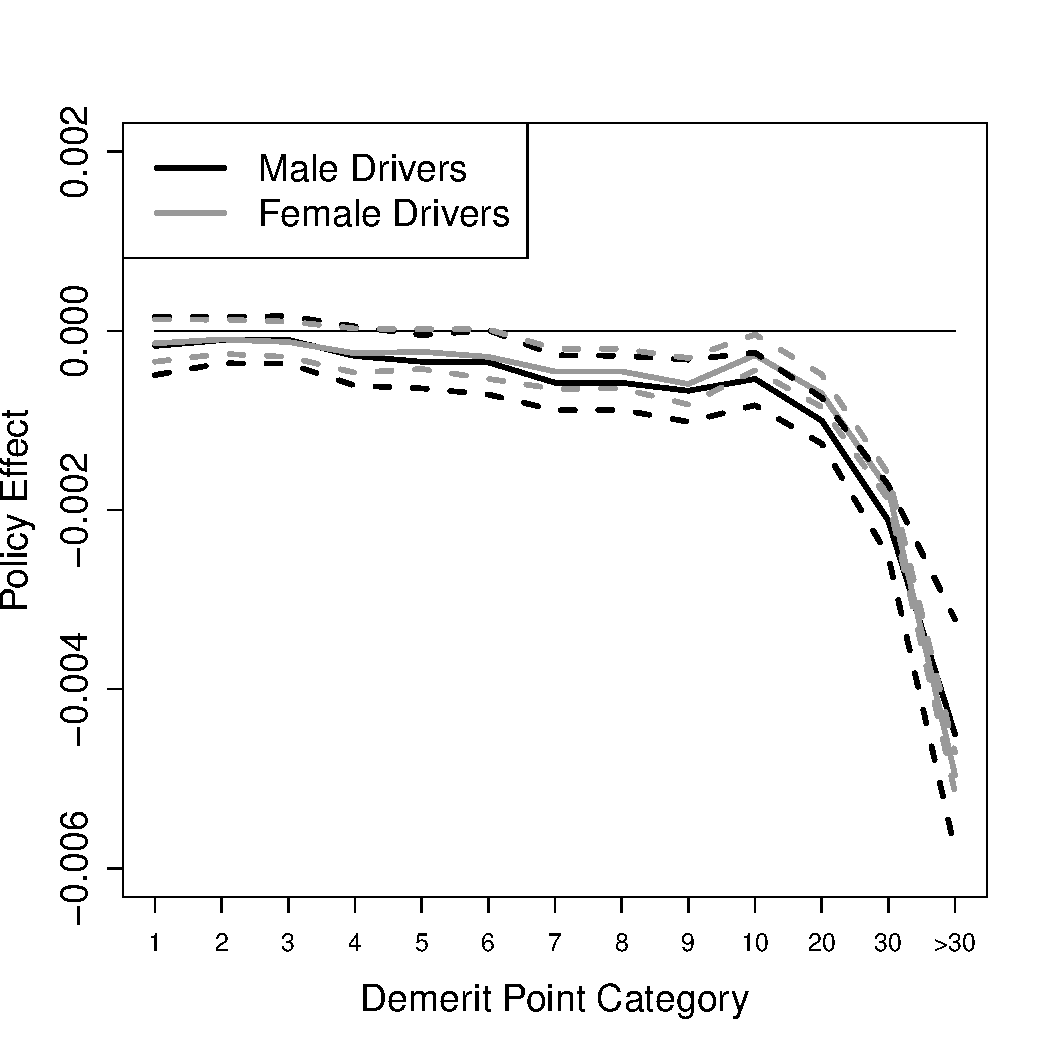
\includegraphics[width=0.8\textwidth]{../Figures/FFX_reg_policy_points_grp_all_pts.pdf}
\caption{Policy change and demerit points group interactions}
%Coefficients on the interaction term between the change in the policy 
%by the current demerit points category of each driver.
%Estimates were calculated by fitting a fixed effects regression model, 
%with intercept coefficients for each driver. 
%% 
%Policy effects for male drivers are shown in black and those for females are shown in grey. 
%% 
%The dashed lines indicate upper and lower 95\% confidence intervals. }
% 
\label{fig:FE_regs_all_pts}
\end{figure}


\clearpage
\pagebreak
\subsection*{High-Point Drivers}




% Fixed Effects Regression Models (drivers with high demerit-point balances) 

\begin{table}% [ht] 
\centering 
\begin{tabular}{l r r r r r r} 

\hline 
 

Sample 
 & \multicolumn{2}{c}{All  Drivers}  & \multicolumn{2}{c}{Male  Drivers}  & \multicolumn{2}{c}{Female  Drivers}   \\ 
 

 \cmidrule(lr){1-1}\cmidrule(lr){2-3}\cmidrule(lr){4-5}\cmidrule(lr){6-7} 

Estimate  & Coefficient & Std. Error  & Coefficient & Std. Error  & Coefficient & Std. Error   \\ 
 

\hline 
 
Intercept  & -0.000  &  0.002  &  0.000  &  0.002  & -0.000  &  0.004   \\ 
 
policy  &  0.126  &  0.007  &  0.116  &  0.008  &  0.161  &  0.013   \\ 
 

\hline 
 
\multicolumn{4}{l}{\textbf{Demerit points group indicators:}}  \\ 
 
1 points  & -0.447  &  0.027  & -0.444  &  0.031  & -0.464  &  0.056   \\ 
 
2 points  & -0.530  &  0.012  & -0.515  &  0.014  & -0.591  &  0.024   \\ 
 
3 points  & -0.490  &  0.010  & -0.500  &  0.011  & -0.451  &  0.019   \\ 
 
4 points  & -0.911  &  0.019  & -0.901  &  0.021  & -0.961  &  0.038   \\ 
 
5 points  & -0.945  &  0.014  & -0.920  &  0.015  & -1.069  &  0.028   \\ 
 
6 points  & -0.868  &  0.013  & -0.892  &  0.014  & -0.769  &  0.025   \\ 
 
7 points  & -1.194  &  0.019  & -1.186  &  0.021  & -1.245  &  0.041   \\ 
 
8 points  & -1.356  &  0.017  & -1.350  &  0.019  & -1.395  &  0.037   \\ 
 
9 points  & -1.253  &  0.018  & -1.299  &  0.020  & -1.023  &  0.038   \\ 
 
10 points  & -1.756  &  0.025  & -1.750  &  0.028  & -1.810  &  0.064   \\ 
 
11-20 points  & -2.153  &  0.016  & -2.144  &  0.017  & -2.250  &  0.041   \\ 
 
21-30 points  & -2.378  &  0.053  & -2.371  &  0.056  & -2.531  &  0.223   \\ 
 
31-150 points  & -1.886  &  0.122  & -1.902  &  0.128  & -1.435  &  0.569   \\ 
 

\hline 
 
\multicolumn{4}{l}{\textbf{Policy and points group interactions:}}  \\ 
 
1 points  & -0.321  &  0.036  & -0.299  &  0.041  & -0.402  &  0.071   \\ 
 
2 points  & -0.219  &  0.016  & -0.218  &  0.019  & -0.221  &  0.031   \\ 
 
3 points  & -0.297  &  0.014  & -0.277  &  0.016  & -0.380  &  0.027   \\ 
 
4 points  & -0.587  &  0.025  & -0.572  &  0.028  & -0.645  &  0.051   \\ 
 
5 points  & -0.553  &  0.018  & -0.556  &  0.021  & -0.530  &  0.039   \\ 
 
6 points  & -0.786  &  0.019  & -0.762  &  0.021  & -0.874  &  0.040   \\ 
 
7 points  & -1.042  &  0.027  & -1.031  &  0.030  & -1.094  &  0.061   \\ 
 
8 points  & -1.019  &  0.025  & -1.009  &  0.027  & -1.058  &  0.057   \\ 
 
9 points  & -1.300  &  0.027  & -1.238  &  0.030  & -1.619  &  0.064   \\ 
 
10 points  & -1.232  &  0.035  & -1.226  &  0.039  & -1.242  &  0.091   \\ 
 
11-20 points  & -1.685  &  0.020  & -1.685  &  0.022  & -1.627  &  0.056   \\ 
 
21-30 points  & -3.123  &  0.068  & -3.120  &  0.072  & -3.013  &  0.289   \\ 
 
31-150 points  & -5.586  &  0.150  & -5.547  &  0.157  & -6.534  &  0.744   \\ 
 

\hline 
 

Drivers 
 & \multicolumn{2}{r}{265,083}  & \multicolumn{2}{r}{214,936}  & \multicolumn{2}{r}{50,147}   \\ 
 

Driver days 
 & \multicolumn{2}{r}{387,028,979}  & \multicolumn{2}{r}{313,813,645}  & \multicolumn{2}{r}{73,215,334}   \\ 
 

SSR 
 & \multicolumn{2}{r}{1,111,029}  & \multicolumn{2}{r}{955,252}  & \multicolumn{2}{r}{155,832}   \\ 
 

\hline 
 
\end{tabular} 
\caption{Fixed effects regression models (drivers with high demerit-point balances)} 
Fixed effects regression coefficients after estimating driver-specific intercept coefficients. 
Samples are drawn by randomly selecting seventy per cent of the drivers. 
\label{tab:FE_regs_high_pts} 
\end{table} 
 





%% Results of F-test for equality of parameters by gender 


We calculated the $F$-statistic to test the restriction 
that the parameters are the same for both male and female drivers. 
The unrestricted sum of squared residuals was 1,111,084. 
The restricted sum of squared residuals was 1,111,029. 
The value of the $F$-statistic was -683, 
which corresponds to a $p$-value of nearly zero, since the $F$-statistic is much higher than 
 the one percent critical value of 1.4763. 
This strongly suggests that male and female driving behaviour should be modeled separately. 




\begin{figure}
\centering
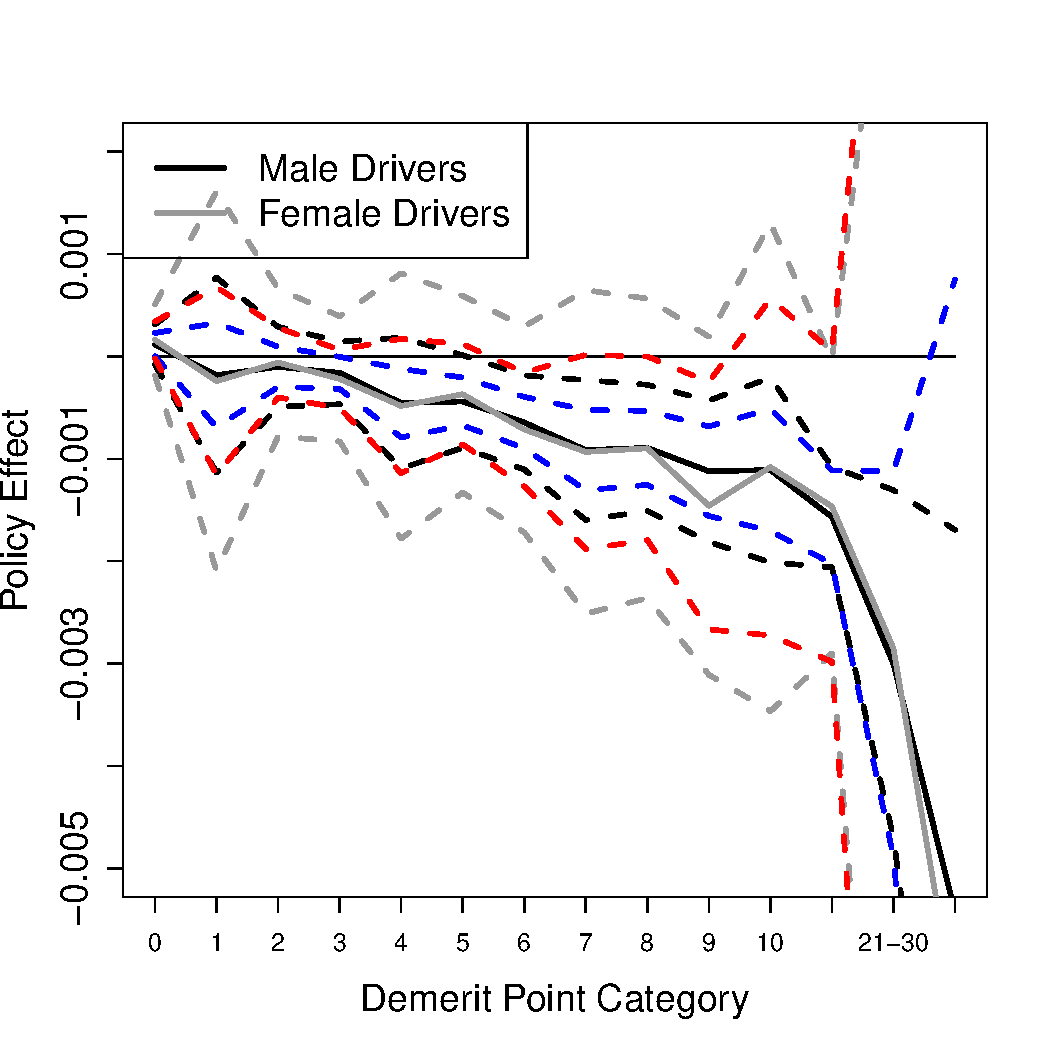
\includegraphics[width=0.8\textwidth]{../Figures/FFX_reg_policy_points_grp_high_pts.pdf}
\caption{Policy change and demerit points group interactions}
%Coefficients on the interaction term between the change in the policy 
%by the current demerit points category of each driver.
%Estimates were calculated by fitting a fixed effects regression model, 
%with intercept coefficients for each driver. 
%% 
%Policy effects for male drivers are shown in black and those for females are shown in grey. 
%% 
%The dashed lines indicate upper and lower 95\% confidence intervals. }
% 
\label{fig:FE-regs}
\end{figure}







\end{document}
